\documentclass[tikz,border=0pt]{standalone}
\usepackage{circuitikz}

\begin{document}

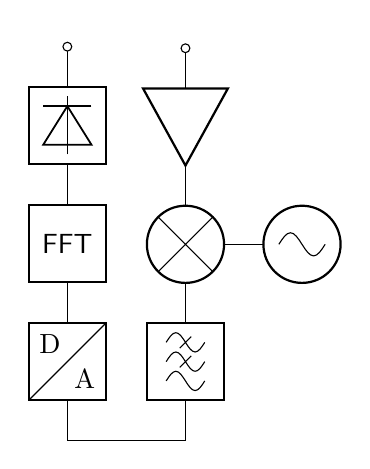
\begin{tikzpicture}
\draw (0,0) node[above]{} to[amp, o-] (0,-2) node[mixer,anchor=north](Q1){};
\draw (Q1.south) to[lowpass] ++(0,-2) to[coordinate] ++(-.75,0) to[coordinate] ++(-.75,0) to[adc] ++(0,+2) to[fft] ++(0,+1) to[detector,-o] ++(0,+2) node[above]{};
\draw (Q1.east) to ++(+.5,0) node[oscillator,anchor=west]{};
\end{tikzpicture}
\vspace{5mm}

\end{document}
